\subsection{Space-time diagrams}
Consider one spatial dimension \(x\) and one temporal dimention \(t\) in an inertial frame \(S\).
We can plot \(x\) on the horizontal axis and \(ct\) on the vertical axis, in order to make the units match.
This combination of space and time in one diagram is called Minkowski spacetime.
Each point \(P\) in spacetime represents an event labelled by coordinates \((x, ct)\).
A moving particle traces out a curve in this diagram, called the world line.
\begin{center}
	\begin{tikzpicture}
		\begin{axis}[
				axis lines = left,
				xlabel = \(x\),
				ylabel = \(ct\),
				xtick=\empty,
				ytick=\empty,
			]

			\fill (axis cs:2,1) circle[radius=2pt];
			\node[anchor=south] at (axis cs:2,1) {\(P\)};

			\addplot[domain=0:3, samples=500] {0.5*x + 0.03*sin(deg((pi * x)^(1.5)))};
		\end{axis}
	\end{tikzpicture}
\end{center}
The world line would be a straight line if the particle is moving at a constant velocity.
In particular, light rays have gradient 1.
Since particles cannot travel faster than the speed of light, world lines are restricted to certain regions (drawn in red) of the space time plane, given that the particle is at \(x=0\) when \(t=0\).
\begin{center}
	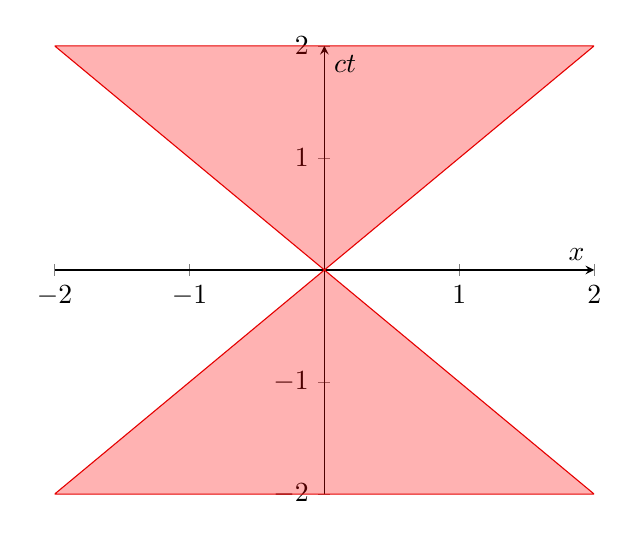
\begin{tikzpicture}
		\begin{axis}[
				axis lines = center,
				xlabel = \(x\),
				ylabel = \(ct\),
			]

			\addplot [red!90!black, fill=red, fill opacity=0.3] coordinates {
					(0, 0) (2, 2) (-2, 2) (2, -2) (-2, -2)
				} -- cycle;
		\end{axis}
	\end{tikzpicture}
\end{center}
We can also draw the axes of a different frame \(S'\) on the same diagram, moving at speed \(v\) relative to \(S\).
The \(t'\) axis corresponds to the equation \(x'=0\) and therefore corresponds to \(x=vt\), or equivalently \(x = \frac{v}{c} \cdot ct\).
The \(x'\) axis corresponds to \(t'=0\), which is \(ct = \frac{v}{c}\cdot x\).
\begin{center}
	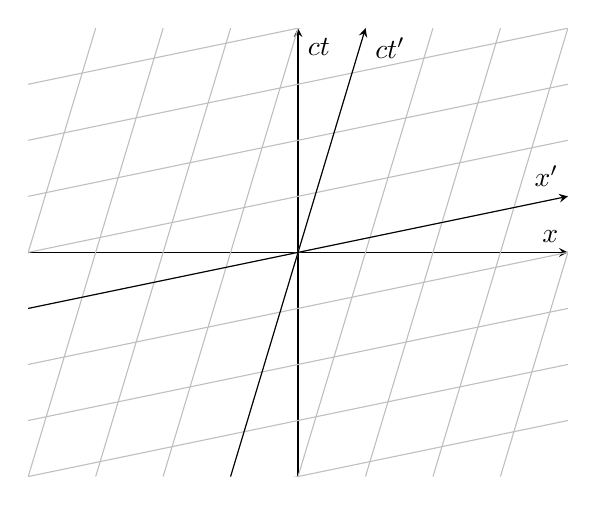
\begin{tikzpicture}
		\begin{axis}[
				axis lines = center,
				xlabel = \(x\),
				ylabel = \(ct\),
				xmin=-2,
				ymin=-2,
				xmax=2,
				ymax=2,
				xtick=\empty,
				ytick=\empty,
			]

			\draw[color=lightgray] (axis cs: -2.5, -2) -- (axis cs: -1.5, 2);
			\draw[color=lightgray] (axis cs: -2, -2) -- (axis cs: -1, 2);
			\draw[color=lightgray] (axis cs: -1.5, -2) -- (axis cs: -0.5, 2);
			\draw[color=lightgray] (axis cs: -1, -2) -- (axis cs: 0, 2);
			\draw[color=lightgray] (axis cs: -0.5, -2) -- (axis cs: 0.5, 2);
			\draw[color=lightgray] (axis cs: 0, -2) -- (axis cs: 1, 2);
			\draw[color=lightgray] (axis cs: 0.5, -2) -- (axis cs: 1.5, 2);
			\draw[color=lightgray] (axis cs: 1, -2) -- (axis cs: 2, 2);
			\draw[color=lightgray] (axis cs: 1.5, -2) -- (axis cs: 2.5, 2);

			\draw[color=lightgray] (axis cs: -2, -2.5) -- (axis cs: 2, -1.5);
			\draw[color=lightgray] (axis cs: -2, -2) -- (axis cs: 2, -1);
			\draw[color=lightgray] (axis cs: -2, -1.5) -- (axis cs: 2, -0.5);
			\draw[color=lightgray] (axis cs: -2, -1) -- (axis cs: 2, 0);
			\draw[color=lightgray] (axis cs: -2, -0.5) -- (axis cs: 2, 0.5);
			\draw[color=lightgray] (axis cs: -2, 0) -- (axis cs: 2, 1);
			\draw[color=lightgray] (axis cs: -2, 0.5) -- (axis cs: 2, 1.5);
			\draw[color=lightgray] (axis cs: -2, 1) -- (axis cs: 2, 2);
			\draw[color=lightgray] (axis cs: -2, 1.5) -- (axis cs: 2, 2.5);

			\draw[->,>=stealth] (axis cs: -0.5, -2) -- (axis cs: 0.5, 2);
			\node[anchor=north west] at (axis cs:0.5,2) {\(ct'\)};
			\draw[->,>=stealth] (axis cs: -2, -0.5) -- (axis cs: 2, 0.5);
			\node[anchor=south east] at (axis cs:2,0.5) {\(x'\)};

		\end{axis}
	\end{tikzpicture}
\end{center}
The angle between the \(x\) and \(x'\) axes matches the angle between the \(ct\) and \(ct'\) axes; they are symmetric about the diagonal (as are the original \(x\) and \(ct\) axes).
Note that the diagonal is given by \(x=ct\) and \(x'=ct'\), which is the same light ray.

\subsection{Comparing velocities}
Consider a particle moving with constant velocity \(u'\) in \(S'\), where \(S'\) is travelling at velocity \(v\) with respect to \(S\).
The world line of the particle in \(S'\) is simply \(x' = u' t'\).
Correspondingly in \(S\), \(x=ut\).
Now, using the Lorentz transformation,
\[
	x=\gamma(x' + vt') = \gamma(u' + v)t'
\]
\[
	t = \gamma\qty(t' + \frac{vx'}{c^2}) = \gamma\qty(1 + \frac{vu'}{c^2})t'
\]
Hence,
\[
	u = \frac{x}{t} = \frac{u' + v}{1 + \frac{u'v}{c^2}}
\]
Note that
\[
	c-u = \frac{(c - u')(c - v)}{1 + \frac{u' v}{c^2}}
\]
which is always positive if \(u'<c\) and \(v<c\).
Therefore, a Lorentz transformation preserves the property that a speed is smaller than the speed of light.

\subsection{Simultaneity}
Two events \(P_1\) and \(P_2\) are simultaneous in \(S\) if they occur at the same time in \(S\).
This is a line parallel to the space axis in the spacetime diagram.
In another reference frame, this line of constant time might be at a different angle.
So events simultaneous in \(S'\) may not correspond to events simultaneous in \(S\).
We can use the above formulae to deduce the exact time that an event happens in a different frame of reference.

\subsection{Causality}
Different observers may disagree on the time ordering of events, but we can construct a viewpoint which gives a consistent description of `cause' and `effect', so special relativity does not break causality.
Note that lines of simultaneity cannot have an angle greater than \(\frac{\pi}{2}\) since the speed of the moving frame must be less than \(c\).
We can construct a `light cone' from all lines or surfaces from an event \(P\) at an angle \(\frac{\pi}{2}\) to the time axis, which represents the possible effects of an event.
\begin{center}
	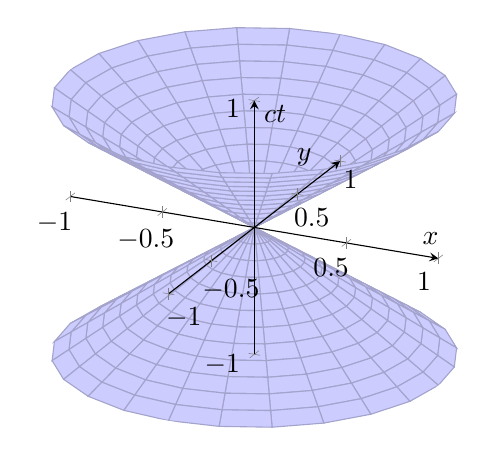
\begin{tikzpicture}
		\begin{axis}[
				axis lines=center,
				axis on top,
				%plot box ratio=1 1 1,
				xlabel=\(x\),
				ylabel=\(y\),
				zlabel={\(ct\)},
				%shader=flat,
				colormap={blue}{rgb=(0.8,0.8,1.0) rgb=(0.8,0.8,1.0)}
			]
			\addplot3 [surf, domain=-1:1, y domain=0:2*pi, z buffer=sort, colormap name=blue] ({x*cos(deg(y))},{x*sin(deg(y))},{x});
		\end{axis}
	\end{tikzpicture}
\end{center}
The cone above the origin is the `future light cone' and the cone below is called the `past light cone'.
Note that this cone is fixed under Lorentz transformations.
If an event occurs in the future light cone, then all observers agree that this event occurs after that the event at the origin.
Likewise, if an event occurs in the past light cone, all observers agree that this event occurs before the event at the origin.
Note that if an event \(P\) is not in the light cone, then it cannot cause, or be caused by, the event at the origin, since nothing travels faster than \(c\).
Hence, an event at the origin can only be influenced by events inside the past light cone, and may only influence events inside the future light cone.

\subsection{Time dilation}
Consider first a clock which is stationary in \(S'\), which ticks at constant intervals \(\Delta t'\).
What is the time interval between ticks as perceived in \(S\)?
We can use the Lorentz transformation, noting that \(x'=0\) since the clock is stationary in \(S'\), to get
\[
	t = \gamma\qty(t' + \frac{vx'}{c^2}) = \gamma t'
\]
Hence,
\[
	\Delta t = \gamma \Delta t'
\]
So moving clocks run slowly.

\subsection{The twin paradox}
Consider two twins \(A\) and \(B\).
Twin \(A\) stays on Earth (considered to be an inertial frame), and \(B\) travels at a constant speed \(v\) to a distant planet \(P\), then she turns around and returns to Earth.
In the frame of reference of \(A\),
\begin{center}
	\begin{tikzpicture}
		\begin{axis}[
				axis lines = left,
				xlabel = \(x\),
				ylabel = \(ct\),
				xtick=\empty,
				ytick=\empty,
				width=4cm,
				height=10cm,
				xmin=0,
				xmax=2.5,
				ymin=0,
				ymax=5,
			]

			%\fill (axis cs:2,1) circle[radius=2pt];
			\node[anchor=south] at (axis cs:1,0) {\(P\)};
			\node[anchor=west] at (axis cs:1,2) {\(E\)};
			\node[anchor=west] at (axis cs:0,4) {\(F\)};
			\draw[dashed,color=lightgray] (axis cs: 1, 0) -- (axis cs: 1, 5);

			\draw[->-=0.5] (axis cs: 0, 0) -- (axis cs: 1, 2);
			\draw[->-=0.5] (axis cs: 1, 2) -- (axis cs: 0, 4);
		\end{axis}
	\end{tikzpicture}
\end{center}
\(E\) is the point where \(B\) reaches \(P\).
The event \(E\) occurs at time \(T\) as perceived by \(A\), so \(E\) has coordinates \((x, ct) = (vT, cT)\).
The time experienced by \(B\) on her outward journey is
\[
	T' = \gamma\qty(T - \frac{v}{c}\cdot vT) = \frac{T}{\gamma}
\]
On her return to event \(F\), twin \(A\) has aged by \(2T\) but twin \(B\) has aged by \(2T' < 2T\).
However, from twin \(B\)'s perspective, twin \(A\) has aged less than she has, since the problem is seemingly symmetric.
This would be a paradox.
To rectify this, consider the frame of reference of \(B\)'s outward journey.
At \(E\), \(x' = 0\) and \(t' = T / \gamma\).
Consider an event \(G\) simultaneous to \(E\) in the frame of reference of \(S'\).
The blue line is a line of constant \(t'\).
\begin{center}
	\begin{tikzpicture}
		\begin{axis}[
				axis lines = left,
				xlabel = \(x\),
				ylabel = \(ct\),
				xtick=\empty,
				ytick=\empty,
				width=4cm,
				height=10cm,
				xmin=0,
				xmax=2.5,
				ymin=0,
				ymax=5,
			]

			%\fill (axis cs:2,1) circle[radius=2pt];
			\node[anchor=south] at (axis cs:1,0) {\(P\)};
			\node[anchor=north west] at (axis cs:1,2) {\(E\)};
			\draw[dashed,color=lightgray] (axis cs: 1, 0) -- (axis cs: 1, 5);
			\draw[color=blue] (axis cs: 0, 1.75) -- (axis cs: 2, 2.25);
			\node[blue,anchor=north west] at (axis cs:0,1.75) {\(G\)};

			\draw[->-=0.5] (axis cs: 0, 0) -- (axis cs: 1, 2);
			\draw[->-=0.5] (axis cs: 1, 2) -- (axis cs: 0, 4);
		\end{axis}
	\end{tikzpicture}
\end{center}
At \(E\),
\[
	t' = \gamma\qty(t - \frac{vx}{c^2}) = t\gamma \implies t = \frac{t'}{\gamma} = \frac{T}{\gamma^2}
\]
So each of them thinks that the other has aged less, when \(B\) is at \(E\), by a factor of \(\gamma^{-1}\).
On the return,
\begin{center}
	\begin{tikzpicture}
		\begin{axis}[
				axis lines = left,
				xlabel = \(x\),
				ylabel = \(ct\),
				xtick=\empty,
				ytick=\empty,
				width=4cm,
				height=10cm,
				xmin=0,
				xmax=2.5,
				ymin=0,
				ymax=5,
			]

			%\fill (axis cs:2,1) circle[radius=2pt];
			\node[anchor=south] at (axis cs:1,0) {\(P\)};
			\node[anchor=west,xshift=0.4cm] at (axis cs:1,2) {\(E\)};
			\draw[dashed,color=lightgray] (axis cs: 1, 0) -- (axis cs: 1, 5);
			\draw[color=red] (axis cs: 0, 2.25) -- (axis cs: 2, 1.75);
			\node[red,anchor=south west] at (axis cs:0,2.25) {\(H\)};
			\draw[color=blue] (axis cs: 0, 1.75) -- (axis cs: 2, 2.25);
			\node[blue,anchor=north west] at (axis cs:0,1.75) {\(G\)};

			\draw[->-=0.5] (axis cs: 0, 0) -- (axis cs: 1, 2);
			\draw[->-=0.5] (axis cs: 1, 2) -- (axis cs: 0, 4);
		\end{axis}
	\end{tikzpicture}
\end{center}
The red line is a line of constant \(t'\) as measured by \(B\) on the return journey, at \(E\).
So for the return journey, \(A\) sees \(B\) age from the event \(E\) to the event \(F\).
However, \(B\) sees \(A\) age from the event \(H\) to the event \(F\).
So there is a time gap between \(G\) and \(H\) as observed by \(B\), which is not considered by the naive model of this problem.
\(B\) sees \(A\) age instantaneously at the point when she changes direction.
In particular, the frame of \(B\) as she changes direction is not inertial.

\subsection{Length contraction}
The length of an object is dependent on the choice of frame.
Consider a rod of length \(L'\) in \(S'\), which is stationary in \(S'\).
The world lines of the ends of the rod are vertical.
The length of the rod at time \(t'\) is the distance in \(x'\) between the two world lines.
In \(S\),
\[
	x' = 0 \implies \gamma(x - vt) = 0
\]
Further,
\[
	x' = L' \implies \gamma(x - vt) = L'
\]
Therefore, the distance between the two \(x\) points at the same \(t\) is \(L = L'/\gamma < L'\).
So the length of a moving object shrinks in the direction it is moving.
Sometimes, analogously to `proper time', we consider the `proper length' of an object, which is the length as measured in the rest frame of the object.

For example, does a train of (proper) length \(2L\) fit alongside a platform of length \(L\) if it is travelling along the tracks at a speed such that \(\gamma = 2\)?
For observers on the platform, the train indeed contracts to length \(L\), so indeed it fits.
On the other hand, for observers on the train, the platform contracts to a length \(\frac{1}{2}L\), so the train would not fit.
To resolve the uncertainty, we will draw a spacetime diagram, from the frame of reference \(S\) where the platform is stationary.
The red lines represent the end points of the platform.
The world lines for the end points of the train are in blue.
\(E\) is the event when the rear of the train is at the rear of the platform, and \(F\) is the event where the front of the train is at the front of the platform.
\begin{center}
	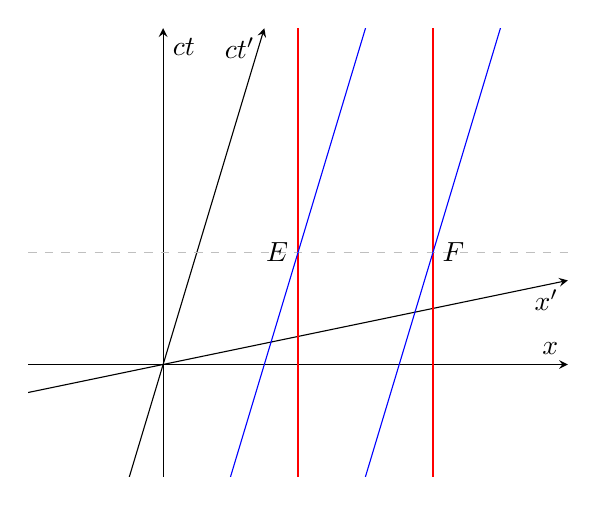
\begin{tikzpicture}
		\begin{axis}[
				axis lines = center,
				xlabel = \(x\),
				ylabel = \(ct\),
				xtick=\empty,
				ytick=\empty,
				xmin=-1,
				xmax=3,
				ymin=-1,
				ymax=3,
			]

			\draw[->,>=stealth] (axis cs: -0.5, -2) -- (axis cs: 0.75, 3);
			\node[anchor=north east] at (axis cs:0.75,3) {\(ct'\)};
			\draw[->,>=stealth] (axis cs: -2, -0.5) -- (axis cs: 3, 0.75);
			\node[anchor=north east] at (axis cs:3,0.75) {\(x'\)};

			\draw[color=red] (axis cs: 1, -1) -- (axis cs: 1, 3);
			\draw[color=red] (axis cs: 2, -1) -- (axis cs: 2, 3);

			\draw[dashed,color=lightgray] (axis cs: -1, 1) -- (axis cs: 3, 1);
			\node[anchor=east] at (axis cs:1, 1) {\(E\)};
			\node[anchor=west] at (axis cs:2, 1) {\(F\)};

			\draw[color=blue] (axis cs: 0, -3) -- (axis cs: 2, 5);
			\draw[color=blue] (axis cs: 1, -3) -- (axis cs: 3, 5);

			%\draw[dashed,color=lightgray] (axis cs: 1, 0) -- (axis cs: 2, 5);
		\end{axis}
	\end{tikzpicture}
\end{center}
Let \(E\) correspond to \(t = 0\) and \(t' = 0\).
The front of the train is at \(x' = 2L\), and the front of the platform is at \(x = L\).
In the \(S\) frame, events \(E\) and \(F\) occur at the same time \(t = 0\).
\[
	x' = \gamma(x - vt) \implies 2L = \gamma(L - vt) = 2(L - vt) \implies t = 0
\]
Further,
\[
	x = \gamma(x' + vt') \implies L = \gamma(2L + vt') = 2(2L + vt') \implies t' = \frac{L - 4 L}{2v} = \frac{-3L}{2v} < 0
\]
Hence, the time \(t'\) at which \(F\) occurs is before the event \(E\).
So from the perspective of the train, the front of the train has already passed the front of the platform by the time that the back of the train passes the back of the platform, so from this perspective the train does not fit.
